\documentclass[aspectratio=169,11pt]{beamer}

\usetheme{Madrid}
\usecolortheme{whale}
\setbeamertemplate{navigation symbols}{}
\setbeamertemplate{footline}[frame number]

\usepackage{amsmath,amssymb}
\usepackage{booktabs}
\usepackage{tikz}
\usetikzlibrary{shapes.geometric, arrows.meta, positioning, fit, calc}
\usepackage{graphicx}

\title{\textbf{AutoCloud-Agent}\\Multi-Agent RL for Cloud Resource Management}
\subtitle{Resource Management in the Cloud for Elasticity and Cost Minimization}
\author{Cloud Computing Term Project}
\institute{Indian Institute of Technology Kharagpur}
\date{March 2026}

\begin{document}

% Slide 1: Title
\begin{frame}
\titlepage
\end{frame}

% Slide 2: Problem Statement
\begin{frame}{Problem Statement}
\textbf{Goal:} Manage cloud VMs to optimize two competing objectives:

\vspace{0.3cm}
\begin{columns}[T]
\begin{column}{0.48\textwidth}
\textbf{Elasticity}
\begin{itemize}
  \item Scale up fast when demand spikes
  \item Maintain SLA (P95 latency $<$ 500ms)
  \item Handle VM boot delay (30--90s)
\end{itemize}
\end{column}
\begin{column}{0.48\textwidth}
\textbf{Cost Minimization}
\begin{itemize}
  \item Scale down idle VMs aggressively
  \item Avoid paying for unused resources
  \item Pack jobs onto fewer machines
\end{itemize}
\end{column}
\end{columns}

\vspace{0.5cm}
\textbf{Limitations of existing approaches:}
\begin{itemize}
  \item Kubernetes HPA / AWS Auto Scaling: reactive, not proactive
  \item Single-agent RL: combinatorial action space ($\sim$15M combinations)
\end{itemize}
\end{frame}

% Slide 3: Our Approach
\begin{frame}{Our Approach: Multi-Agent Decomposition}
\textbf{Key idea:} Split resource management into 3 independent sub-problems,
each handled by a separate PPO agent.

\vspace{0.3cm}
\begin{center}
\begin{tabular}{lccc}
\toprule
\textbf{Agent} & \textbf{Action} & \textbf{Frequency} & \textbf{Action Space} \\
\midrule
ScaleOut & Add/remove VMs & Every 10 steps (5 min) & 3 \\
Consolidation & Drain idle VMs & Every 2 steps (1 min) & $2^{20}$ \\
Scheduling & Assign job priority & Every step (30s) & 5 \\
\bottomrule
\end{tabular}
\end{center}

\vspace{0.3cm}
\textbf{Result:} Joint space $3 \times 2^{20} \times 5 \approx 15$M
$\rightarrow$ Three manageable independent spaces.
\end{frame}

% Slide 4: Architecture
\begin{frame}{System Architecture}
\begin{center}
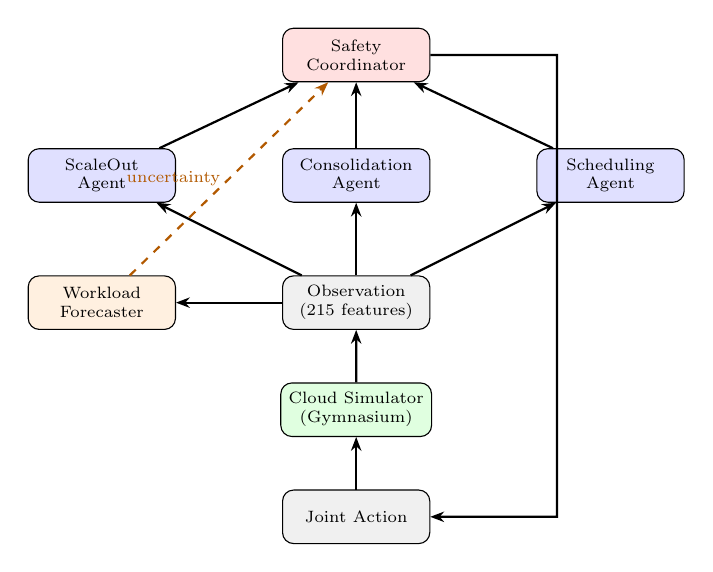
\begin{tikzpicture}[
  block/.style={rectangle, draw, rounded corners, minimum height=0.8cm,
    minimum width=2.2cm, align=center, font=\scriptsize},
  agent/.style={block, fill=blue!12},
  sim/.style={block, fill=green!12},
  fore/.style={block, fill=orange!12},
  coord/.style={block, fill=red!12},
  arrow/.style={-{Stealth[length=5pt]}, thick},
  every node/.style={font=\scriptsize},
  scale=0.85, transform shape
]

\node[sim] (env) at (0,0) {Cloud Simulator\\(Gymnasium)};
\node[block, fill=gray!12] (obs) at (0,1.6) {Observation\\(215 features)};
\node[agent] (so) at (-3.8,3.5) {ScaleOut\\Agent};
\node[agent] (con) at (0,3.5) {Consolidation\\Agent};
\node[agent] (sch) at (3.8,3.5) {Scheduling\\Agent};
\node[fore] (fc) at (-3.8,1.6) {Workload\\Forecaster};
\node[coord] (safety) at (0,5.3) {Safety\\Coordinator};
\node[block, fill=gray!12] (act) at (0,-1.6) {Joint Action};

\draw[arrow] (env) -- (obs);
\draw[arrow] (obs) -- (so);
\draw[arrow] (obs) -- (con);
\draw[arrow] (obs) -- (sch);
\draw[arrow] (obs) -- (fc);
\draw[arrow] (so) -- (safety);
\draw[arrow] (con) -- (safety);
\draw[arrow] (sch) -- (safety);
\draw[arrow, dashed, orange!70!black] (fc) -- node[left]{uncertainty} (safety);
\draw[arrow] (safety) -- ++(3,0) |- (act);
\draw[arrow] (act) -- (env);
\end{tikzpicture}
\end{center}
\end{frame}

% Slide 5: RL Algorithm
\begin{frame}{RL Algorithm: Independent PPO (I-PPO)}
Each agent uses Proximal Policy Optimization [Schulman et al., 2017]:

\[
  L^{\text{CLIP}} = \mathbb{E}\left[\min\left(
    r_t \hat{A}_t,\;
    \text{clip}(r_t, 1{-}\epsilon, 1{+}\epsilon)\,\hat{A}_t
  \right)\right]
\]

\begin{columns}[T]
\begin{column}{0.48\textwidth}
\textbf{Network:}
\begin{itemize}
  \item 3-layer MLP + LayerNorm
  \item 512 $\to$ 256 $\to$ 128 $\to$ action
  \item Separate actor \& critic
\end{itemize}
\end{column}
\begin{column}{0.48\textwidth}
\textbf{Hyperparameters:}
\begin{itemize}
  \item $\gamma = 0.99$, $\lambda = 0.95$
  \item Clip $\epsilon = 0.2$
  \item LR: $3 \times 10^{-4}$ (Adam)
  \item Entropy: $0.01 \to 0.001$
\end{itemize}
\end{column}
\end{columns}

\vspace{0.3cm}
\textbf{Agent-specific rewards:} ScaleOut (provisioning cost + SLA), Consolidation (running cost + migration), Scheduling (wait time + SLA)
\end{frame}

% Slide 6: Forecaster
\begin{frame}{Workload Forecaster: Transformer + MC Dropout}
\begin{columns}[T]
\begin{column}{0.55\textwidth}
\textbf{Input:} 20 time steps $\times$ 4 features\\
(CPU, queue length, hour, day-of-week)

\vspace{0.3cm}
\textbf{Architecture:}
\begin{itemize}
  \item 2-layer Transformer encoder
  \item 4 attention heads, 64-dim hidden
  \item Quantile regression (10th, 50th, 90th)
\end{itemize}

\vspace{0.3cm}
\textbf{Uncertainty [Gal \& Ghahramani, 2016]:}
\begin{itemize}
  \item 30 stochastic forward passes
  \item MC Dropout $\to$ variance = uncertainty $\sigma$
  \item Cheaper than ensemble ($5\times$ fewer params)
\end{itemize}
\end{column}
\begin{column}{0.43\textwidth}
\textbf{Predictions:}
\begin{itemize}
  \item $t{+}1$, $t{+}5$, $t{+}10$, $t{+}15$
  \item 3 quantiles each
  \item Uncertainty $\sigma$ per horizon
\end{itemize}

\vspace{0.3cm}
\textbf{What it enables:}
\begin{itemize}
  \item Proactive scaling (pre-boot VMs)
  \item Safety: if $\sigma > 0.3$, suppress draining
  \item Better resource planning
\end{itemize}
\end{column}
\end{columns}
\end{frame}

% Slide 7: Safety Coordinator
\begin{frame}{Safety Coordinator}
Rule-based post-processing filter. Guarantees safety regardless of policy quality.

\vspace{0.3cm}
\begin{center}
\begin{tabular}{clp{7cm}}
\toprule
\textbf{\#} & \textbf{Filter} & \textbf{Rule} \\
\midrule
1 & Boot Protection & Never drain a node younger than boot\_time + 60s \\
2 & $N_{\min}$ Floor & Never go below 3 active nodes \\
3 & Uncertainty Suppression & If $\sigma > 0.3$, block all drain actions \\
4 & Scale-Out Suppression & Block scale-up if $\geq$2 nodes booting \\
5 & Proactive Scale-Out & If $\sigma > 0.3$ AND CPU rising, force +1 \\
\bottomrule
\end{tabular}
\end{center}

\vspace{0.3cm}
\textbf{Why separate from reward?}\\
Hard constraints in rewards only penalize violations --- they don't prevent them.
The coordinator \textit{guarantees} constraint satisfaction.
\end{frame}

% Slide 8: Simulator
\begin{frame}{Cloud Simulator}
Custom SimPy-based discrete-event simulator with Gymnasium API.

\vspace{0.3cm}
\begin{columns}[T]
\begin{column}{0.48\textwidth}
\textbf{Configuration:}
\begin{itemize}
  \item 3--20 VMs, 4 node types
  \item 30s time step, 120 steps/episode
  \item Node lifecycle: BOOTING $\to$ ACTIVE $\to$ DRAINING $\to$ TERMINATED
\end{itemize}
\end{column}
\begin{column}{0.48\textwidth}
\textbf{Observation (215-dim):}
\begin{itemize}
  \item 120: node features (20$\times$6)
  \item 80: job features (20$\times$4)
  \item 15: global (CPU, queue, forecast)
\end{itemize}
\end{column}
\end{columns}

\vspace{0.3cm}
\textbf{Workload:} Alibaba Cluster Trace 2018 [Alibaba, 2018]\\
4,023 machines, 7 days of production data, binned at 30s intervals.
\end{frame}

% Slide 9: Results
\begin{frame}{Results}
\begin{center}
\begin{tabular}{lcccc}
\toprule
\textbf{Method} & \textbf{SLA} & \textbf{Cost Eff.} & \textbf{CPU Util.} & \textbf{Stability} \\
\midrule
\textbf{AutoCloud-Agent} & \textbf{100\%} & \textbf{0.962} & \textbf{0.552} & 0.889 \\
MPCController & 100\% & 0.962 & 0.552 & 0.941 \\
ThresholdReactive & 100\% & 0.955 & 0.483 & 0.822 \\
StaticN & 100\% & 0.938 & 0.333 & 1.000 \\
KubernetesHPA & 100\% & 0.930 & 0.312 & 0.842 \\
AWSTargetTracking & 100\% & 0.928 & 0.295 & 0.876 \\
SingleAgentPPO & 100\% & 0.924 & 0.413 & 0.794 \\
\bottomrule
\end{tabular}
\end{center}

\vspace{0.3cm}
\begin{itemize}
  \item Matches MPC on cost efficiency (0.962), the best classical method
  \item 3.4\% better than Kubernetes HPA on cost
  \item CPU utilization nearly $2\times$ that of AWS Target Tracking
  \item Multi-agent outperforms single-agent by 4.1\% cost, 33.7\% CPU
\end{itemize}
\end{frame}

% Slide 10: Ablation & Stress Testing
\begin{frame}{Ablation Study \& Stress Testing}
\begin{columns}[T]
\begin{column}{0.48\textwidth}
\textbf{Why multi-agent wins:}
\begin{itemize}
  \item SingleAgentPPO: 0.924 cost, 41.3\% CPU
  \item AutoCloud: 0.962 cost, 55.2\% CPU
  \item Temporal hierarchy: each agent matches its natural decision frequency
  \item Per-agent rewards: clearer learning signal
\end{itemize}
\end{column}
\begin{column}{0.48\textwidth}
\textbf{Stress scenarios:}
\begin{enumerate}
  \item Ramp-up (20\%\,$\to$\,100\%)
  \item Sudden spike (30\%\,$\to$\,95\% in 5 steps)
  \item Choppy plateau (70--90\% + noise)
  \item Trough-then-recovery
\end{enumerate}
\vspace{0.2cm}
Safety Filter 5 (proactive scale-out) is critical for sudden spike: forces +1 node when $\sigma > 0.3$ and CPU rising.
\end{column}
\end{columns}
\end{frame}

% Slide 11: Limitations & Future Work
\begin{frame}{Limitations \& Future Work}
\begin{columns}[T]
\begin{column}{0.48\textwidth}
\textbf{Current limitations:}
\begin{itemize}
  \item Homogeneous VMs only
  \item Single-cluster scope
  \item Simplified networking
  \item Static reward weights
  \item Single-day training data
\end{itemize}
\end{column}
\begin{column}{0.48\textwidth}
\textbf{Future work:}
\begin{itemize}
  \item Heterogeneous VM types
  \item Multi-cluster federation
  \item Vertical scaling (VM resizing)
  \item Transfer learning across traces
  \item Spot instance pricing
\end{itemize}
\end{column}
\end{columns}
\end{frame}

% Slide 12: Conclusion
\begin{frame}{Conclusion}
\textbf{AutoCloud-Agent} decomposes cloud resource management into three
independent RL agents with:

\vspace{0.3cm}
\begin{enumerate}
  \item \textbf{Multi-agent I-PPO:} 3 agents at different temporal frequencies
  \item \textbf{Uncertainty-aware forecasting:} Transformer + MC Dropout for proactive scaling
  \item \textbf{Safety coordinator:} 5 hard-constraint filters guaranteeing system stability
\end{enumerate}

\vspace{0.3cm}
\textbf{Key results:}
\begin{itemize}
  \item 96.2\% cost efficiency (matches MPC, beats HPA by 3.4\%)
  \item 55.2\% CPU utilization ($2\times$ AWS Target Tracking)
  \item 100\% SLA compliance
  \item 4.1\% cost and 33.7\% CPU improvement over single-agent RL
\end{itemize}

\vspace{0.3cm}
\textbf{References:} Schulman et al. (PPO, 2017), Vaswani et al. (Transformers, 2017), Gal \& Ghahramani (MC Dropout, 2016), Zhang et al. (AWARE, USENIX ATC 2023)
\end{frame}

\end{document}
